\begin{figure}[H]
\centering
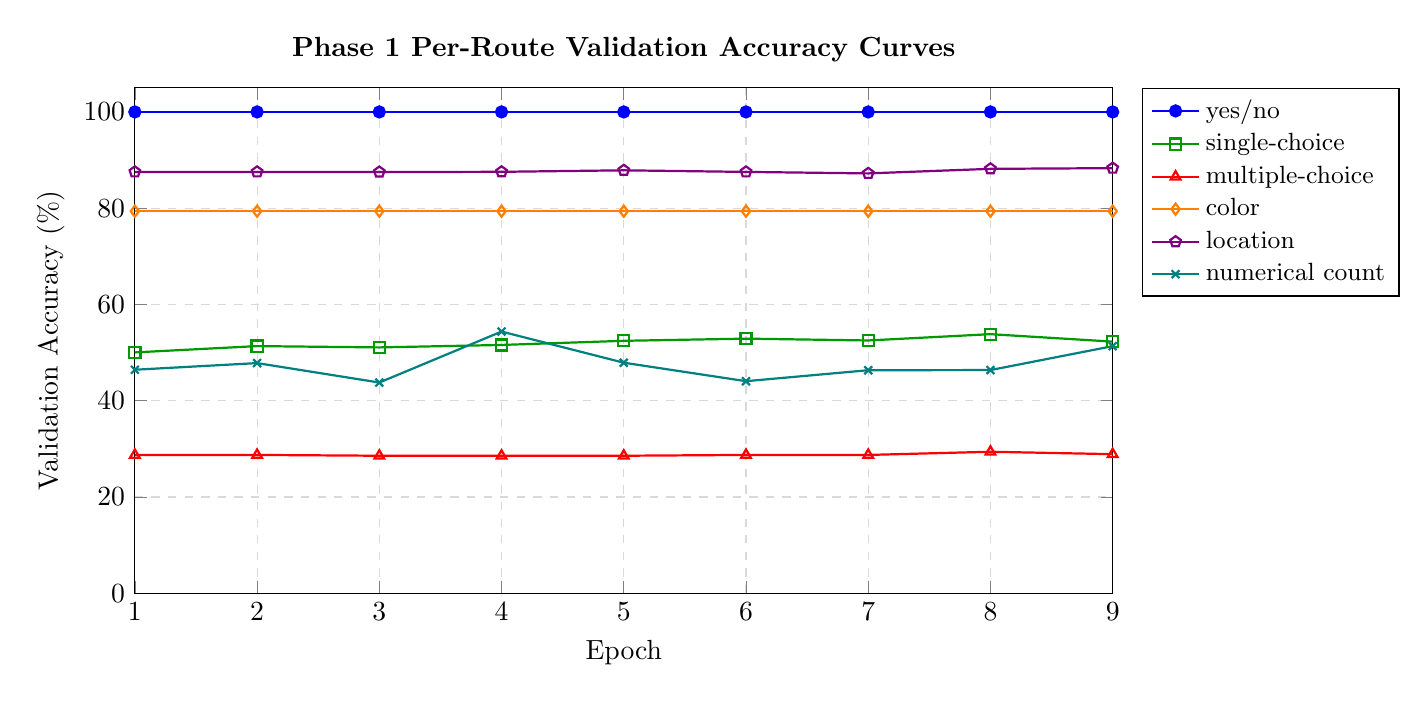
\begin{tikzpicture}
\begin{axis}[
    width=14cm, height=8cm,
    xlabel={Epoch}, ylabel={Validation Accuracy (\%)},
    xmin=1, xmax=9, ymin=0, ymax=105,
    grid=major, grid style={dashed,gray!30},
    legend pos=outer north east, legend cell align=left,
    legend style={font=\small},
    title={\textbf{Phase 1 Per-Route Validation Accuracy Curves}},
]
\addplot[blue, thick, mark=*]
  coordinates {(1,100.00) (2,100.00) (3,100.00) (4,100.00) (5,100.00) (6,100.00) (7,100.00) (8,100.00) (9,100.00)};
\addlegendentry{yes/no}
\addplot[green!60!black, thick, mark=square]
  coordinates {(1,50.04) (2,51.35) (3,51.08) (4,51.59) (5,52.45) (6,52.90) (7,52.52) (8,53.83) (9,52.28)};
\addlegendentry{single-choice}
\addplot[red, thick, mark=triangle]
  coordinates {(1,28.74) (2,28.74) (3,28.57) (4,28.57) (5,28.57) (6,28.74) (7,28.74) (8,29.40) (9,28.90)};
\addlegendentry{multiple-choice}
\addplot[orange, thick, mark=diamond]
  coordinates {(1,79.38) (2,79.38) (3,79.38) (4,79.38) (5,79.38) (6,79.38) (7,79.38) (8,79.38) (9,79.38)};
\addlegendentry{color}
\addplot[violet, thick, mark=pentagon]
  coordinates {(1,87.54) (2,87.54) (3,87.51) (4,87.56) (5,87.87) (6,87.54) (7,87.23) (8,88.18) (9,88.32)};
\addlegendentry{location}
\addplot[teal, thick, mark=x]
  coordinates {(1,46.44) (2,47.82) (3,43.78) (4,54.37) (5,47.90) (6,44.06) (7,46.34) (8,46.37) (9,51.34)};
\addlegendentry{numerical count}
\end{axis}
\end{tikzpicture}
\caption{Phase 1 per-route validation accuracy across 9 epochs. Yes/No
saturates immediately; Single Choice and Multi Choice show slow improvement;
Colour and Location are stable; Count fluctuates due to ordinal granularity.}
\label{fig:p1_per_route_val}
\end{figure}
